\documentclass[11pt]{article}
% Language setting
\usepackage[spanish]{babel}
\usepackage[capposition=top]{floatrow}
\usepackage{booktabs}
\usepackage{tabularx}
\usepackage{array}
\usepackage{caption}
\usepackage{multirow}
\usepackage{makecell}

% Set page size and margins
\usepackage[a4paper,top=2cm,bottom=2cm,left=3cm,right=3cm,marginparwidth=1.75cm]{geometry}

% Used packages
\usepackage{amsmath}
\usepackage{graphicx}
\usepackage[colorlinks=true, allcolors=blue]{hyperref}
\usepackage{apacite}
\usepackage{booktabs}

\DeclareMathOperator*{\argminA}{arg\,min}

% Keywords command
\providecommand{\keywords}[1]
{
  \small	
  \textbf{\textit{Keywords}} #1
}

\newcommand{\source}[1]{\vspace{-4pt}{\footnotesize{Fuente: {#1}} } }

\title{Efectos del uso de redes sociales sobre el bienestar subjetivo en contexto de aislamiento social}
\author{Leonardo A. Caravaggio}
\date{}
\begin{document}
\maketitle

\begin{abstract}
Con la irrupción de la pandemia de COVID-19 se produjo un fuerte proceso de digitalización de la vida, por medidas restrictivas y decisiones de cuidado. El impacto del uso de redes sociales en el bienestar está relacionado con el contexto del uso. En el presente trabajo se analiza el impacto causal del uso de redes sociales en el bienestar subjetivo de la población latinoamericana durante la pandemia. Se utiliza un modelo de regresión cuantílica con variables instrumentales, lo que permite considerar el efecto causal y evitar la endogeneidad de ambas variables (utilizando la calidad del acceso a internet como instrumento), y el impacto a lo largo de la distribución de bienestar, lo que permite identificar efectos asimétricos. Si bien en general el impacto del uso de redes sociales sobre el bienestar subjetivo es negativo, también se observa que para las personas con menor bienestar subjetivo, durante el contexto particular de la pandemia, fue positivo. 
\end{abstract}

\keywords{Felicidad, Bienestar, Redes Sociales, COVID-19, IVQR}

\section{Introducción}
La irrupción de la pandemia de COVID-19 y las diferentes estrategias de aislamiento generaron un proceso de aceleración de la digitalización de las tareas y las relaciones interpersonales. Más personas comenzaron a utilizar redes sociales. Usar redes sociales tiene efectos en el bienestar de las personas, en particular en su bienestar subjetivo ($SWB$, por sus siglas en inglés). Esos efectos no son siempre iguales, sino que dependen del tipo de uso. En general, durante la pandemia, se hizo un uso de redes sociales que no reemplaza relaciones cara a cara posibles, sino que hace posible mantener el contacto con otros en una situación en la que de otra forma no hubiera sido posible. El uso de redes sociales en ese contexto resulta especialmente de interés. El efecto positivo encontrado para los de menor $SWB$ se explica en que las relaciones cara a cara no eran posibles. 

Existe a su vez otra motivación para analizar el caso particular de la pandemia: los vínculos que el $SWB$ tiene sobre el bienestar objetivo. En particular en un contexto de pandemia resulta interesante que la población no reduzca su $SWB$. Una persona deprimida o con menor $SWB$ tendrá menos razones para cuidarse y cuidar a los demás, será más propensa a enfermarse, etc. Esto a su vez agrava la sobrecarga del sistema de salud. 

Muchas políticas públicas pueden implementarse para aprovechar el vínculo entre la tecnología y el bienestar, sin embargo, se precisa una mejor comprensión de los mecanismos internos para determinar cuál de estas será la mejor. Por ejemplo, se podría promover el acceso a dispositivos entre la población de menos recursos, o difundir capacitación para el uso y aprovechamiento de las redes sociales direccionada especialmente a ciertos sectores, advirtiendo sobre los riesgos posibles, etc. 

La pregunta de investigación del presente trabajo podría plantearse entonces de la siguiente manera: ¿Qué impacto tuvo el uso de redes sociales en el $SWB$ de la población durante la pandemia? ¿Existen diferencias de impacto entre las personas con mayor o menor $SWB$? Estas diferencias de impacto podrían deberse a los diferenciales que las personas con mayor o menor $SWB$ tengan en la posibilidad de generar vínculos sociales reales, especialmente en un contexto de aislamiento. Es decir, las personas podrían usar las redes sociales para generar nuevos vínculos o mantener los existentes o simplemente para aislarse de los demás. En general el primer uso estaría vinculado a una mejora en el $SWB$ y el segundo a un empeoramiento. Así expresado la pregunta sería si las personas con mayor o menor bienestar hacen usos distintos de las redes sociales. También podría pensarse en una competencia entre un efecto positivo y un efecto negativo por el uso de redes sociales. El primero vinculado a las relaciones sociales y los vínculos con los demás, y el segundo a los efectos nocivos que el uso (o mal uso) genera. 

Pueden mencionarse dos efectos contrarios del uso de redes sociales sobre el $SWB$. El primero, un efecto negativo. Esto podría deberse a que provocan envidia o comparación social. Las redes sociales ponen en contacto a las personas con lo que otros muestran en sus perfiles, lo que generalmente es la mejor parte de sus vidas. Esto podría inducir a envidiar los viajes, los amigos, la comida y en general la vida que otros disfrutan, haciendo ver la propia vida como menos satisfactoria y por tanto reduciendo el propio $SWB$. El uso de redes sociales podría provocar también aislamiento. Es más fácil pasar la tarde \textit{scrolleando} con el celular que entablar un diálogo real con los demás. Sin embargo, a largo plazo, esto podría ir en detrimento de la calidad y la cantidad de los vínculos sociales reales. También podría producirse un efecto de fatiga, especialmente entre las personas que se quedan hasta tarde en las redes sociales en detrimento de las horas de sueño. O de pérdida de productividad, por distracción en el trabajo, etc.

El segundo, un efecto positivo, por interacción social. Las redes sociales permiten comunicarse y vincularse con otros, lo que claramente está relacionado con una mejora en el $SWB$. Supóngase, por ejemplo, el caso de una madre que siente menos el peso de la migración de su hijo a otro continente por la posibilidad de ``seguirlo'' en redes sociales. Pero el contexto importa ya que, para que el uso de redes sociales tenga un efecto positivo en el $SWB$ el mismo no debe reemplazar a relaciones sociales reales posibles (consumo de bienes relacionales), sino que debe ser utilizado como un sustituto cuando estas resulten imposibles o demasiado costosas. En el contexto de aislamiento producto de la pandemia estos efectos de reemplazo de relaciones sociales posibles, son especialmente interesantes. Al resultar muy difícil encontrarse con otros, ya sea por cuestiones legales o decisiones personales, las redes sociales podrían presentar un buen sustituto en la vinculación interpersonal. En este caso no se estaría reemplazando una relación real posible por una virtual, sino que simplemente el uso de red social podría haber hecho posible un vínculo y una cercanía con los otros. 

Cabe mencionar que podría observarse una bidireccionalidad en la relación. Las personas que se reconocen a sí mismas como felices podrían tener más razones para hacer uso de redes sociales, porque disponen de más tiempo, quieren mostrarle a otros lo felices que son, etc. O tal vez, las personas menos felices podrían tener razones para hacer más uso de las redes sociales, porque están solas y solo encuentran satisfacción pasajera en la distracción que las redes sociales generan. También podría ser que las personas más felices tengan menos razones para hacer uso de redes sociales, por ejemplo porque encuentran una satisfacción más duradera con su familia y amigos en vínculo directo, o en otras actividades. Lo mismo las menos felices, por ejemplo porque están tan deprimidas que no les interesa enterarse de la vida de los otros. 

Por otro lado, los efectos del uso de redes sociales podrían ser disímiles para las personas más o menos felices. Por ejemplo una persona deprimida, con pocos vínculos sociales reales, podría usar la tecnología simplemente para evadirse de la realidad, sin lograr con la misma generar vínculos reales y por tanto sin afectar su bienestar, o afectándolo negativamente. Otra con mejor respuesta subjetiva y vínculos reales podría aprovechar la tecnología para mantenerse en contacto con sus amigos y familia. O una persona con poca interacción social real podría al menos sacar provecho de las relaciones sociales virtuales, logrando un mejor efecto por su uso que una persona con mayor $SWB$. 

Para investigar estas relaciones, se utiliza un modelo de variables instrumentales por cuantiles. Esto permite indagar el efecto causal del uso de redes sociales sobre el $SWB$ a lo largo de la distribución. Se utiliza como instrumento una variable que capta la calidad del acceso a internet en la zona de residencia del encuestado. 

El trabajo se estructura de la siguiente manera: en la próxima sección se presentan los antecedes bibliográficos, luego se discute en mayor profundidad la problemática y el objetivo propuestos. En una sección independiente se presenta la estrategia empírica y los datos utilizados, y en otra los resultados. Por último, las conclusiones. 

\section{Literatura Previa}

El campo de estudio de la felicidad en economía recibe aportes provenientes de distintas ramas del conocimiento. Con causas y consecuencias de alto impacto para la teoría económica, también resulta un tema cercano a la psicología, la medicina, la sociología, etc. La economía de la felicidad utiliza como medida de bienestar el $SBW$. Incluso algunos autores lo proponen como el fin último de la economía utilitarista. Es decir, lo interpretan directamente como la utilidad percibida por las personas \cite{Easterlin2021}. Si bien esta interpretación tiene sus limitaciones y problemas, el diagnóstico que la persona haga de su propio bienestar parece irreemplazable por otro indicador económico u objetivo y por tanto resulta de mucho valor. A su vez, la relación entre $SWB$ y otros indicadores de objetivos de bienestar permiten hacer una valoración en sí misma del primero. Por ejemplo en cuanto las personas más satisfechas con su vida o más felices resultan más saludables \cite{STEPTOE2015640, Diener2011}, o más productivas \cite{Oswald2009}. Una reseña bibliográfica de los impactos del uso de estos indicadores subjetivos de bienestar en economía puede verse en \citeA{Rojas2019} o en \citeA{Bruni2007}. Si bien este trabajo no indaga más allá de la respuesta subjetiva, no debe olvidarse que la misma es importante no solo en sí misma, sino también por sus efectos de segunda vuelta. 

Respecto de la relación entre el uso de redes sociales y $SWB$, distintos trabajos encontraron resultados disímiles de acuerdo al contexto. Por ejemplo, \citeA{Verduyn2017} observan una caída en el $SWB$ por el uso pasivo de redes sociales, por envidia y comparación social. \citeA{Wadhwa2019} ponen el acento en este mismo fenómeno como consecuencia de la pérdida de sueño, productividad y motivación generado por el uso de tecnologías de la información. \citeA{Wirtz2021} encuentran que el uso de redes sociales tiene efectos negativos sobre el $SWB$ especialmente en las situaciones en las que el uso de redes sociales sustituye a las vinculaciones reales. Es decir, si el uso que se le da a las redes sociales es solo para ver la vida de los otros, como distracción y como evasión, el mismo produce efectos negativos en el bienestar. En esta línea pueden verse, entre otros, los trabajos de \citeA{Zhou2019} o \citeA{Wenninger2019}. 

Por el contrario, el uso activo de las redes sociales podría aumentar el $SWB$. Esto podría deberse a que el mismo permite la creación de capital social y estimula los sentimientos de conexión social \cite{Easterlin2021}. El uso de redes sociales puede ayudar a generar nuevos vínculos o a mantener vínculos con personas que están lejos, o resulta imposible ver seguido. Los resultados y la interpretación de \citeA{Winstead2013} van en esta línea. 

El tipo de uso que se le de a la red social es fundamental para determinar el  efecto en $SWB$. Esta tensión puede verse por ejemplo en \citeA{Antoci2018}. También se observa en los adultos mayores que aprovechan la tecnología para reducir su soledad, como muestran \citeA{Lelkes2013} y \citeA{Richter2013} con datos de europa, \citeA{Choi2009} con datos de Estados Unidos, o \citeA{Lu2021} con datos de China. \citeA{Clark2017} proponen una división entre quienes usan las redes sociales para interactuar con otros, y por tanto generar nuevos vínculos reales o sostener los existentes y quienes solo utilizan las redes sociales para observar la vida de los demás, pero sin vinculación real. Esto puede verse también en el trabajo que presenta \citeA{Khalaila2018} con redes sociales o \citeA{Bruni2008} con la televisión. En general, reemplazar el consumo de bienes relacionales por otros menos costosos puede resultar satisfactorio en el corto plazo, pero no en el mediano plazo. 

Diferentes tipos de personas hacen usos diferentes de las redes sociales. Un ejemplo de esto es la diferenciación por edad. Por ejemplo, \citeA{Verduyn2017} muestran que el uso de redes sociales afecta positivamente al $SWB$, pero no en forma directa sino atenuando el impacto de la perdida de capacidades de los adultos mayores. Es decir, el impacto del uso de redes sociales es especialmente positivo para quienes tienen mayor dificultad para acceder a los vínculos sociales en forma directa. \citeA{Kim2017} señalan que entre los jóvenes el uso de redes sociales ayuda a generar vínculos sociales reales. \citeA{Webster2021} reseñan distintos estudios en la relación de redes sociales y $SWB$ en adolescentes. En general encuentran que las relaciones sociales cara a cara tienen mejores efectos que el uso de redes sociales. Se advierte especialmente en este rango etário un efecto negativo frente a la satisfacción con el propio cuerpo, por efecto de la envidia y las críticas recibidas. Un tercer grupo de estudio posible es el del efecto del uso de redes sociales en los menores de edad. Por sus características particulares los impactos en la socialización y el bienestar emocional puede entendiblemente separarse del promedio poblacional general. \citeA{McDool2016} analizan este caso. 

Algunos estudios incluso encuentran que el uso de redes sociales no afecta al bienestar. Pueden verse ejemplos de esto en \citeA{10.1093/jcmc/zmaa014} y \citeA{Orben2019}. Esto podría deberse a una cancelación de los distintos efectos en una determinada población. Por ejemplo, en los estudios que al analizar el uso de redes sociales no discriminan entre distintos tipos de redes sociales. Algunas redes sociales tienen como principal objetivo la comunicación con personas conocidas (p.e. Whatsapp). Otras favorecen el intercambio de noticias y opiniones principalmente con desconocidos (p.e. Twitter). Otras permiten ver qué están haciendo los demás ya sea vínculos cercanos (p.e. Facebook) o sumando también a famosos (p.e. Instagram). Otras buscan maximizar el tiempo que las personas pasan en la red social mostrando contenido atractivo ya sea de conocidos o desconocidos (p.e. Snapchat, Tiktok o incluso Youtube). El diseño y objetivo de la red social seguramente esté relacionado con el tipo de uso que hace la persona. Una persona que solo usa Whatsapp presumiblemente tenga mejores vínculos reales que una persona que solo usa Tiktok. 

Estos diferentes usos no solo tendrán diferentes efectos en el $SWB$ sino también en otros aspectos de la vida. Es esperable, por ejemplo, que las redes sociales que generan mayor adicción induzcan más a las personas a quedarse enganchados hasta tarde en detrimento de las horas de sueño (p.e. Tiktok). Otras redes, por su uso y función podrían provocar mayores distracciones durante el trabajo (p.e. Whatsapp o Twitter). También podría pensarse en un grupo de redes que por su forma tengan mayores impactos en las expectativas y la conformidad con la propia vida (p.e. Instagram). 

Más en general \citeA{Valkenburg2022} ofrece una importante reseña del impacto del uso de redes sociales no solo en el bienestar (por ejemplo $SWB$) sino también en el malestar (por ejemplo la depresión). Los artículos allí comentados se clasifican de acuerdo al criterio antedicho considerando los efectos del uso activo (por ejemplo postear contenido) o pasivo (solo mirar) de redes sociales. \citeA{Schoenning2020} también reseñan los artículos en esta dirección, con especial foco en los adolescentes. Ellos advierten que muchos estudios analizan no solo el uso o no uso de redes sociales, sino también la cantidad de tiempo dedicado a esto. Esta problemática resulta de especial interés para el caso de los adolescentes. Cabe destacar que no pareciera conllevar el mismo resultado una gran cantidad de tiempo utilizado en uso pasivo de redes sociales que el utilizado en un uso activo de las mismas (\citeA{Bekalu2019} hablan incluso de un uso saludable y uno nocivo de redes sociales relacionado con la vinculación afectiva generada por el uso y la integración del mismo con la socialización real). Por el contrario sí se detallan en esta segunda reseña la diferenciación entre los estudios por el bienestar y el malestar (a este respecto ver también \citeA{Yang2022}). 

Debiera advertirse también que el uso de redes sociales puede tener otros efectos que generen impactos de segunda vuelta en el bienestar. Por ejemplo, las redes sociales, ya sea por publicidad o por imitación del consumo de otros, invitan a realizar determinados consumos. Estos consumos luego tendrán también un impacto sobre el $SWB$. \citeA{Ho2019} estudian estos efectos. 

Una línea de investigación interesante es preguntarse qué tipo de mecanismos podrían implementarse para evitar o reducir los efectos nocivos del uso de redes sociales, sin perder sus efectos negativos. \citeA{Lambert2022} estudian los efectos positivos de evitar el uso de redes sociales durante una semana. Esta técnica permitiría evitar al menos por un tiempo la influencia de los efectos de la envidia por comparación social, o los incentivos al consumo superfluo, mejorar el descanso, sin perder vínculos sociales reales. 

\section{El impacto del uso de redes sociales en el bienestar subjetivo}
El impacto del uso de redes sociales en las personas es relevante en al menos dos sentidos. Por un lado, por los diversos efectos que este uso de redes sociales tiene en el $SWB$ de la población, pero por otro, por los efectos que el $SWB$ tiene en la salud, la productividad y otros resultados objetivos. 

Es de esperar que el impacto que el uso de redes sociales tenga en el $SWB$ sea heterogéneo para distintos cortes poblacionales. Para poder aplicar políticas públicas bien direccionadas será necesario conocer si los efectos son mayores entre los menos o los más felices, entre los más jóvenes o los adultos mayores, los pobres o los ricos, o tantos otros recortes posibles. 

Como ya se mencionó, el uso de redes sociales puede tener dos efectos contrarios sobre el $SWB$. Uno negativo y uno positivo. El positivo principalmente vinculado a la capacidad de poner en contacto a las personas entre sí cuando no es posible hacerlo cara a cara. Esto se da especialmente en poblaciones donde el contacto social es de otra manera más complicado o imposible, por ejemplo en los adultos mayores, la población rural o en los aislados por cuestiones sanitarias. La situación de la pandemia de COVID-19 presenta un caso de estudio particularmente interesante para esto. 

En cambio, si el uso de redes sociales reemplaza vínculos reales posibles podría caerse en una trampa. Las redes sociales generan la sensación de una vinculación real, cuando en realidad, la misma no existe o es menos intensa de lo que parece. Una persona puede tener la sensación de tener un vínculo cercano con otra porque a diario ve fotos suyas y está al tanto de lo que el otro está haciendo. Sin embargo, la otra persona podría ni haberse enterado de que la primera ve las fotos. Además la relación es solo con lo que se sube a las redes y puede no enterarse de los problemas reales del otro.

Uno de los principales determinantes de un buen nivel de $SWB$ es el buen vínculo con la familia, amigos y la sociedad circundante en general. Podría entenderse a este determinante como un gran mediador entre el uso de redes sociales y el $SWB$. Si el uso de redes sociales ayuda a generar, mantener o mejorar vínculos reales y cercanos con personas reales, entonces el uso de redes sociales tendrá efectos positivos en $SWB$. Si el uso de redes sociales produce aislamiento, resentimiento o envidia con los otros, cansancio, etc. lo más probable es que también genere una caída en el $SWB$. 

La relación entre el uso de redes sociales y el $SWB$ podría ser bidireccional. No solo usar redes sociales afecta a la manera en que las personas se sienten, sino que el como se sienten podría inducirlos a usar o no usar redes sociales. Para lograr una identificación causal será necesario entonces el uso de variables instrumentales. Para esto, la calidad del acceso a internet resulta un instrumento útil. La validez de la variable como instrumento del uso de redes sociales ($SNU$ por sus siglas en inglés) se define por su incorrelación con el bienestar subjetivo ($SWB$) y su correlación con $SNU$. Teóricamente su utilización se justifica en que tiene sentido pensar que en los lugares donde la calidad de la conexión a internet sea mejor, las personas utilicen más las redes sociales. Por otro lado, una mejor calidad en la conexión a internet no pareciera tener un vínculo directo con el $SWB$ no mediado por el uso de redes sociales. El estadístico F de Cragg-Donald arroja un resultado de 275.16. El estadístico F del test de Kleibergen-Paap arroja un resultado de 348.53 (p $<$ 0.01), sobre el umbral propuesto por \citeA{lee2022}, lo que permite rechazar la hipótesis nula de debilidad de instrumentos. 

Por otro lado, el uso que las personas más felices hagan de las redes sociales podría ser distintos del uso que hacen los menos felices. Incluso llevando a situaciones en las que en el total poblacional no se observe un efecto. Esta situación podría deberse a una anulación por la contraposición de los distintos efectos producidos por el uso de redes sociales. Es decir que dependiendo el corte que se haga se podría ver que a algunas personas el uso de redes sociales les mejora su bienestar, mientras que a otras se lo empeora, de manera que en el conjunto el efecto total podría ser nulo. Por este motivo resulta particularmente interesante identificar qué cortes poblacionales hacen distinto uso de las redes sociales y por tanto tienen mayor impacto positivo o negativo. Por ejemplo, el análisis a lo largo de la distribución de bienestar. Entendiendo que por los efectos recíprocos entre bienestar y uso de redes sociales, las personas de acuerdo a su bienestar harán distintos usos de las mismas. La metodología de regresiones cuantílicas permite hacer estos análisis sobre la distribución del bienestar, y en el marco de las variables instrumentales resulta útil el modelo de variables instrumentales por cuantiles (IVQR) desarrollado por \citeA{Chernozhukov2005}.


\section{Estrategia empírica y datos}
\subsection{Estrategia Empírica}
A los fines de lograr identificar el efecto causal del uso de redes sociales en el $SWB$ se utilizó en primer lugar una regresión de mínimos cuadrados ordinarios (OLS) y luego una regresión en dos etapas (2SLS) sobre el siguiente modelo: 

 \[SWB_i =  \alpha SNU_i + \gamma X_i + u_i \]

La variable dependiente, $SWB$ intenta aproximar el bienestar subjetivo considerando dos variables subjetivas: la variable de felicidad construida sumarizando distintas preguntas subjetivas sobre bienestar, economía y relaciones sociales ($fel$), y la respuesta a la pregunta por satisfacción con la vida ($sat$). $SNU$ representa a la variable de tratamiento: uso de redes sociales. $X_i$ representa al vector de variables de control: se utilizó la edad y la posibilidad de haber realizado trabajo remoto. $u_i$ es el término de error. 

La regresión de OLS no permite captar el efecto causal del uso de redes sociales sobre el $SWB$ por lo que se implementa la regresión en dos etapas. Se utiliza la calidad de la conexión a internet (\textit{avg\_d\_kbps}) como instrumento (Z). 

\[SNU_i =  \beta Z + \gamma X_i + u_i \]

Se advierte también que los efectos del uso de redes sociales ($SNU$) podrían no estar equitativamente distribuidos sobre la distribución de bienestar de los encuestados. Esto quiere decir que personas con distintos niveles de $SWB$ podrían hacer usos distintos de las redes sociales y por tanto obtener resultados distintos sobre su nivel de $SWB$. Por ejemplo, alguien con elevado nivel de $SWB$ podría usar la red para intercambiar con familiares y amigos, y estaría menos propenso a sufrir efectos de envidia por comparación social, etc. En cambio alguien con menor nivel de $SWB$ si usa la red social podría ayudarlo a deprimirse más al observar cómo los otros la pasan bien, mientras que él permanece aislado, etc. O bien podría darse el caso contrario en el que los que menor bienestar presentan logran con el uso de redes sociales algún tipo de contacto social que les proporciona un beneficio mayor que el que este uso le reporta a los de mayor bienestar. La regresión cuantílica permite identificar estas asimetrías. 

Para incorporar ambos efectos (endogeneidad y asimetría), se utilizó la metodología propuesta por \citeA{Chernozhukov2005} de regresión cuantílica con variables instrumentales (IVQR). Para esto, se siguió la definición de \citeA{Chernozhukov2006, Chernozhukov2008} utilizando la implementación de \citeA{Machado2018}. Es decir, el cuantíl $\tau$-ésimo de la variable dependiente $Q_{SWB} (\tau)$ se estima como una función lineal de la variable endógena ($SNU_i$), el vector de control ($X_i$), y el término de error ($u_i$)

 \[Q_{SWB}(\tau) =  \alpha_\tau SNU_i + \beta_\tau X_i + u_i \]

El estimador de la regresión cuantílica convencional se define como el mejor predictor de $Y=SWB$ dado $X$ bajo la desviación mínima de la función de pérdida: \[\rho_t(u)=(\tau-1(u<0))u\] 

El modelo se describe con mayor detalle en el Anexo Metodológico.  

\subsection{Datos}
Dado que lo que se quiere identificar es el efecto del uso de redes sociales sobre el $SWB$ en el contexto particular de reducción o eliminación de los encuentros cara a cara, se utilizaron datos de la encuesta Latinobarómetro de la ola 2020. Se trata de un estudio de opinión publica que recoge alrededor de 20.000 entrevistas por ola en total en 18 países de América Latina, lo que implica una representación de más de 600 millones de habitantes. Las encuestas de esta ola se realizaron entre Octubre y Diciembre de 2020 (salvo para Argentina que por medidas de aislamiento debió posponerse para Abril y Mayo de 2021) \cite{Latinobarometro2020a, Latinobarometro2020}. En ese período la pandemia de COVID-19 todavía presentaba una elevada cantidad de casos activos de coronavirus SARS-CoV2 en la región, y los distintos países tenían vigentes diferentes medidas preventivas de aislamiento, suspensión de clases, prohibición de espectáculos masivos, etc. Incluso, más allá de estas medidas, muchas personas continuaban evitando el contacto con adultos mayores, reuniones de muchas personas, o muchos empleados continuaban en modalidad de trabajo a distancia con menor contacto con sus compañeros de trabajo, etc.  

La variable independiente del presente estudio es el bienestar subjetivo ($SWB$), entendido en primer término directamente como el nivel de satisfacción subjetiva con la vida. Esta variable  se obtiene con las respuestas a la pregunta subjetiva por satisfacción con la vida: ``En términos generales, ¿diría Ud. que está satisfecho con su vida? ¿Diría Ud. que está....? Muy satisfecho, bastante satisfecho, no muy satisfecho, para nada satisfecho" ($sat$). Esta pregunta se coloca al inicio del cuestionario para evitar sesgos por efectos de estímulos previos (``priming''). La interpretación de la respuesta a la pregunta por la satisfacción con la vida como un nivel general de bienestar subjetivo es común en la literatura. 

En segundo término se aproxima el $SWB$ con un índice que busca captar la felicidad subjetiva ($fel$). Esta variable se creó sumarizando las respuestas a la pregunta por satisfacción con la vida $sat$ con estas otras: ``¿Diría Ud. que este país... está progresando / está estancado / está en retroceso?'' ($progreso$), ``¿Cómo calificaría en general la situación económica actual del país? Muy buena / buena / regular / mala / muy mala" ($eco\_pais$), ``¿Y en los próximos doce meses, cree que su situación económica y la de su familia será mucho mejor, un poco mejor, igual, un poco peor, o mucho peor que la que tiene hoy?'' ($eco\_fliar$) y finalmente ``Hablando en general, ¿Diría Ud. que se puede confiar en la mayoría de las personas o que uno nunca es lo suficientemente cuidadoso en el trato con los demás? Se puede confiar en la mayoría de las personas / Uno nunca es lo suficientemente cuidadoso en el trato con los demás'' ($conf$). Es decir que esta variable de aproximación al $SWB$ tiene en cuenta no solo la satisfacción con la vida, sino también otras consideraciones subjetivas respecto de la situación económica y las relaciones sociales con los demás. Estos temas son, de acuerdo con \citeA{Easterlin2021}, los que más afectan a la felicidad de las personas. Por este motivo se entiende esta segunda variable como un nivel de felicidad de las personas, el cuál también es interpretable como su nivel subjetivo de bienestar. Se recodificó la variable de satisfacción con la vida, de manera que al igual que la variable de felicidad valores más bajos representen menor satisfacción o menor felicidad y valores más altos representen mayor satisfacción o mayor felicidad. Los histogramas de la variable de felicidad ($fel$) y de la variable de satisfacción con la vida ($sat$) pueden verse en el Anexo. 

La variable de tratamiento se genera como una dummy con valor cero cuando el encuestado no refiere utilizar ninguna de las redes sociales que se le muestran luego de la pregunta ``¿Usa Ud. alguno de los siguientes servicios de redes sociales si es que Ud. usa alguno?: Facebook, Whatsapp, Snapchat, Instagram, Youtube, Tik Tok, Twitter, LinkedIn''. Si el encuestado refiere usar una o más de las mencionadas redes sociales, la variable toma valor uno. Así, el grupo de tratamiento consta de 15573 personas entre el total de 19610 observaciones analizadas. Siguiendo las siglas en inglés utilizadas en otros trabajos de la literatura se hace referencia a esta variable como $SNU$ (Social Network Use). 

Esta relación entre bienestar y uso de redes sociales se instrumenta a partir de una medida de calidad en el acceso a internet. En este caso se utilizó la base de \href{https://www.ookla.com/ookla-for-good/open-data}{Ookla} que identifica velocidad promedio de internet y latencia por Quadkey. La información proviene de una de las páginas de análisis de velocidad de ancho de banda más utilizada del mundo, \href{https://www.speedtest.net/}{Speedtest}. La página es propiedad de Ookla. Cuando un usuario entra a la página y hace click en el botón de ``GO'' se calcula la latencia y la velocidad de su conexión a internet. La prueba es sencilla, se envía un paquete de información desde la computadora del usuario hasta los servidores de Ookla en Los Ángeles, Estados Unidos. Cuando el paquete es recibido, se envía una respuesta. Se calcula si hubo pérdidas de información y el tiempo que se tarda en toda la operación. Estos datos pueden resultarle útiles al usuario para analizar el estado actual de su servicio. La página realiza este test unas 20 millones de veces por mes. Luego conserva y disponibiliza la información con fecha, hora y localización de la consulta. Para el presente trabajo se utilizaron datos del segundo trimestre de 2020 de manera que coincidan lo más posible con las fechas de la encuesta. La identificación de latitud y longitud de cada una de las 1372 ciudades incluidas en el Latinobarómetro se realizó en forma automática mediante el \textit{scrapeo} de los datos de \href{http://www.geonames.org}{Geonames}. Es decir, para cado de los nombres de las ciudades que aparecen en la base de datos de Latinobarómetro, se realizó en forma automática una búsqueda de identificación en la página mencionada. Ese valor corresponde a la latitud y longitud en la que se ubica la ciudad. Se realizó una conversión de esos valores a Quadkey para posteriormente hacerlo coincidir con el valor de velocidad y latencia correspondiente a ese Quadkey. Se optó por descartar la latencia y utilizar solamente la velocidad de conexión. La variable generada se denomina \textit{avg\_d\_kbps} y representa el promedio de kilobits por segundo de la conexión a internet registrado en la ciudad de residencia del encuestado. \footnote{El código Python utilizado para esta identificación se encuentra junto con el código STATA de las estimaciones y otros elementos de interés en el repositorio público \url{https://github.com/LCaravaggio/felicidad_y_redes}}

Como variables de control se utilizó la $edad$ del entrevistado y la pregunta: ``¿Esta Ud o alguien de su familia trabajando remotamente , o ha trabajado remotamente vía internet desde su hogar durante esta pandemia?'' identificada con el nombre $remoto$ y tipificada como 2 para quienes responden que no y 1 para quienes responden que sí. Las estadísticas descriptivas de todas las variables utilizadas pueden observarse en el Cuadro 1. 

% Cuadro1
\begin{table}[htbp]
  \centering
  \caption{Estadísticas Descriptivas I}
    \begin{tabular}{rlrrrrr}
          &       & \multicolumn{4}{c}{Total}     &  \\
          &       & \multicolumn{1}{c}{media} & \multicolumn{1}{c}{desvío} & \multicolumn{1}{c}{min} & \multicolumn{1}{c}{max} & \multicolumn{1}{c}{\# true} \\
    \midrule
    \multicolumn{1}{l}{sat} & Satisfación con la vida & \multicolumn{1}{c}{1,90} & \multicolumn{1}{c}{0,87} & \multicolumn{1}{c}{1} & \multicolumn{1}{c}{4} &  \\
    \multicolumn{1}{l}{fel} & Felicidad subjetiva & \multicolumn{1}{c}{9,88} & \multicolumn{1}{c}{2,64} & \multicolumn{1}{c}{1} & \multicolumn{1}{c}{18} &  \\
    \multicolumn{1}{l}{SNU} & Uso de redes sociales & \multicolumn{1}{c}{0,79} & \multicolumn{1}{c}{0,40} & \multicolumn{1}{c}{0} & \multicolumn{1}{c}{1} & \multicolumn{1}{c}{15680} \\
    \multicolumn{1}{l}{eco\_país} & Economía del país & \multicolumn{1}{c}{3,53} & \multicolumn{1}{c}{0,93} & \multicolumn{1}{c}{1} & \multicolumn{1}{c}{5} &  \\
    \multicolumn{1}{l}{progreso} & Progreso del país & \multicolumn{1}{c}{2,10} & \multicolumn{1}{c}{0,90} & \multicolumn{1}{c}{1} & \multicolumn{1}{c}{3} &  \\
    \multicolumn{1}{l}{eco\_fliar} & Economía familiar & \multicolumn{1}{c}{2,60} & \multicolumn{1}{c}{1,10} & \multicolumn{1}{c}{1} & \multicolumn{1}{c}{5} &  \\
    \multicolumn{1}{l}{conf} & Confianza en los demás & \multicolumn{1}{c}{1,86} & \multicolumn{1}{c}{0,33} & \multicolumn{1}{c}{1} & \multicolumn{1}{c}{2} & \multicolumn{1}{c}{2486} \\
    
    \multicolumn{1}{l}{estudio} & Nivel de estudios & \multicolumn{1}{c}{1,04} & \multicolumn{1}{c}{4,32} & \multicolumn{1}{c}{1} & \multicolumn{1}{c}{17} &  \\
    \multicolumn{1}{l}{compu} & Tenencia computadora & \multicolumn{1}{c}{1,57} & \multicolumn{1}{c}{0,49} & \multicolumn{1}{c}{1} & \multicolumn{1}{c}{2} & \multicolumn{1}{c}{13582} \\
    \multicolumn{1}{l}{casa} & Tenencia casa propia & \multicolumn{1}{c}{1,30} & \multicolumn{1}{c}{0,46} & \multicolumn{1}{c}{1} & \multicolumn{1}{c}{2} & \multicolumn{1}{c}{13551} \\
    \multicolumn{1}{l}{clase} & Autopercepción de clase & \multicolumn{1}{c}{3,73} & \multicolumn{1}{c}{0,96} & \multicolumn{1}{c}{1} & \multicolumn{1}{c}{5} &  \\
    \multicolumn{1}{l}{edad} & Edad  & \multicolumn{1}{c}{40,84} & 
    \multicolumn{1}{c}{16,48} & \multicolumn{1}{c}{16} & \multicolumn{1}{c}{100} &  \\
    \multicolumn{1}{l}{remoto} & Trabajo remoto  & \multicolumn{1}{c}{1,65} & 
    \multicolumn{1}{c}{0,47} & \multicolumn{1}{c}{1} & \multicolumn{1}{c}{2} &  \multicolumn{1}{c}{12927}\\
    \multicolumn{1}{l}{avg\_d\_kbps} & Calidad internet  & \multicolumn{1}{c}{30904} & 
    \multicolumn{1}{c}{32568} & \multicolumn{1}{c}{46} & \multicolumn{1}{c}{259191} &  \multicolumn{1}{c}{}\\
    \midrule
         N &      &  &       &       &       & 19749  \\
    
    \floatfoot{Nota: Se presentan las medias, desvíos estándar y valores máximos y mínimos para las variables utilizadas. Para las variables dicotómicas se presenta también la cantidad total de valores positivos. Se observa así, por ejemplo, que entre las 19749 personas encuestadas, 15680 hacen uso de algún tipo de red social pero solo 9618 poseen \textit{smartphone}.}
    \end{tabular}%
  \label{tab:Cuadro1}%
\end{table}%

En el Cuadro 2 se observan las estadísticas descriptivas de las mismas variables para los casos afectados y no afectados por el tratamiento, es decir para quienes declaran usar o no usar redes sociales ($SNU$). Puede observarse que quienes utilizan redes sociales son en promedio más jóvenes y viven en ciudades con mejor conexión a internet. El $SWB$ queda indeterminado, la satisfacción con la vida es mayor para quienes no usan redes sociales, pero la felicidad es mayor para quienes sí las usan. 

Del total de 19749 encuestas analizadas, 15680 declaran utilizar redes sociales (79.4\%)\footnote{Los datos utilizados para el presente trabajo pueden descargarse en forma gratuita de la página oficial de Latinobarómetro: \url{https://www.latinobarometro.org/}.}. 

% Cuadro2
\begin{table}[htbp]
  \centering
  \caption{Estadísticas Descriptivas II}
    \begin{tabular}{lrrrrrrr}
          & \multicolumn{2}{c}{\makecell{Usa redes\\ sociales}} &       & \multicolumn{2}{c}{\makecell{No usa \\redes sociales}} &  & \makecell{Dif.de\\medias}\\
          & \multicolumn{1}{c}{media} & \multicolumn{1}{c}{desvío} & \multicolumn{1}{c}{\# true} & \multicolumn{1}{c}{media} & \multicolumn{1}{c}{desvío} & \multicolumn{1}{c}{\# true} \\
    \midrule
    SNU   & \multicolumn{1}{c}{1,00} & \multicolumn{1}{c}{0,00} &       & \multicolumn{1}{c}{0,00} & \multicolumn{1}{c}{0,00} &  \\
    sat  & \multicolumn{1}{c}{1,86} & \multicolumn{1}{c}{0,84} &       & \multicolumn{1}{c}{2,06} & \multicolumn{1}{c}{0,96} &  &\multicolumn{1}{c}{0,203***}\\
    fel   & \multicolumn{1}{c}{9,97} & \multicolumn{1}{c}{2,60} &       & \multicolumn{1}{c}{9,53} & \multicolumn{1}{c}{2,79} &  &\multicolumn{1}{c}{-0,443***}\\
    \midrule
    eco\_país & \multicolumn{1}{c}{3,55} & \multicolumn{1}{c}{0,93} &       & \multicolumn{1}{c}{3,47} & \multicolumn{1}{c}{0,92} &  &\multicolumn{1}{c}{-0,119***}\\
    progreso  & \multicolumn{1}{c}{2,10} & \multicolumn{1}{c}{0,69} &       & \multicolumn{1}{c}{2,09} & \multicolumn{1}{c}{0,70} &  &\multicolumn{1}{c}{-0,142***}\\
    eco\_fliar & \multicolumn{1}{c}{2,56} & \multicolumn{1}{c}{1,07} &       & \multicolumn{1}{c}{2,41} & \multicolumn{1}{c}{1,56} &  &\multicolumn{1}{c}{0,014***}\\
    conf & \multicolumn{1}{c}{1,87} & \multicolumn{1}{c}{0,33} & \multicolumn{1}{c}{1943} & \multicolumn{1}{c}{1,85} & \multicolumn{1}{c}{0,34} & \multicolumn{1}{c}{543} &\multicolumn{1}{c}{-0,128***}\\
    smart & \multicolumn{1}{c}{1,41} & \multicolumn{1}{c}{0,49} & \multicolumn{1}{c}{9037} & \multicolumn{1}{c}{1,85} & \multicolumn{1}{c}{0,35} & \multicolumn{1}{c}{581} &\multicolumn{1}{c}{0,406***}\\
    estudio   & \multicolumn{1}{c}{11,44} & \multicolumn{1}{c}{3,70} &       & \multicolumn{1}{c}{6,54} & \multicolumn{1}{c}{4,31} &   &\multicolumn{1}{c}{-4,898***}\\
    compu & \multicolumn{1}{c}{1,50} & \multicolumn{1}{c}{0,50} & \multicolumn{1}{c}{10537} & \multicolumn{1}{c}{0,19} & \multicolumn{1}{c}{0,33} & \multicolumn{1}{c}{3045} &\multicolumn{1}{c}{0,364***} \\
    casa & \multicolumn{1}{c}{1,32} & \multicolumn{1}{c}{0,46} & \multicolumn{1}{c}{10511} & \multicolumn{1}{c}{1,24} & \multicolumn{1}{c}{0,43} & \multicolumn{1}{c}{3040} &\multicolumn{1}{c}{-0,073***}\\
    clase    & \multicolumn{1}{c}{3,66} & \multicolumn{1}{c}{0,92} &       & \multicolumn{1}{c}{4,02} & \multicolumn{1}{c}{1,05} &  &\multicolumn{1}{c}{0,141***}\\
    edad  & \multicolumn{1}{c}{37,55} & \multicolumn{1}{c}{14,71} &       & \multicolumn{1}{c}{53,53} & \multicolumn{1}{c}{16,79} &  &\multicolumn{1}{c}{16,003***}\\
    remoto & \multicolumn{1}{c}{1,61} & \multicolumn{1}{c}{0,48} & \multicolumn{1}{c}{12927} & \multicolumn{1}{c}{1,8} & \multicolumn{1}{c}{0,40} & \multicolumn{1}{c}{6822} &\multicolumn{1}{c}{0,183***}\\
    avg\_d\_kbps & \multicolumn{1}{c}{32979} & \multicolumn{1}{c}{33318} & \multicolumn{1}{c}{} & \multicolumn{1}{c}{23205} & \multicolumn{1}{c}{26145} & \multicolumn{1}{c}{} &\multicolumn{1}{c}{-9774,8***}\\
    \midrule
    N     &  &       &  15680     &   &       & 4069  \\
        \floatfoot{Nota: Se presentan las medias y desvíos estándar para los grupos de quienes sí usan y quienes no usan redes sociales. Para las variables dicotómicas se presenta también la cantidad total de valores positivos. Se observa así, por ejemplo, que la media de felicidad es mayor para quienes usan redes sociales, quienes también están más satisfechos con su vida ($p1st$). Se presenta también la diferencia de medias donde el nivel de significancia corresponde al test t. *** p$<$0.01, ** p$<$0.05, * p$<$0.1 En todos los casos se acepta la hipótesis alternativa de una diferencia significativamente diferente de cero.}
    \end{tabular}%
  \label{tab:Cuadro2}%
\end{table}%

\section{Resultados}

\subsection{Resultados principales}

El Cuadro \ref{B} presenta la salida de la regresión simple de mínimos cuadrados ordinarios (MCO), la primera etapa (FS), la segunda etapa (IV) y la estimación de regresiones cuantílicas con variables instrumentales (IVQR) para los cuantiles 25\% (especificación 1), 50\% (especificación 2) y 75\% (especificación 3) con satisfacción con la vida ($sat$) como variable dependiente utilizando la calidad de la conexión a internet (\textit{avg\_d\_kbps}) como instrumento. La primera estimación muestra un coeficiente positivo y significativo, el cuál no debe considerarse válido dado el sesgo producido por endogeneidad. La regresión en dos etapas, en cambio, muestra un coeficiente negativo y significativo. Los más satisfechos con su vida también reciben un impacto negativo por el uso de redes sociales (especificación 3). Es decir, un coeficiente negativo y estadísticamente significativo. Estos son los resultados naturalmente esperables. En condiciones normales, el efecto del uso de redes sociales es negativo. Pareciera que para este sector de la distribución de satisfacción los efectos de envidia y adicción prevalecen por sobre los otros. 

Para las especificación de los menos satisfechos con su vida y la mediana se observa, en cambio, que el uso de redes sociales aumenta la probabilidad de que el encuestado se perciba más satisfecho con su vida. Es decir, un coeficiente positivo y estadísticamente significativo. Este resultado se encuentra en línea con el de \citeA{Lu2021} para adultos mayores. Esto se interpreta como una prevalencia de los efectos de la posibilidad de comunicación con amigos y familiares por sobre los de la envidia, adicción y otros negativos en el contexto de la pandemia. Podría pensarse que justamente los menos satisfechos con su vida fueron los que más sufrieron el aislamiento y lograron, al menos, sacar provecho del uso de redes sociales. 

\begin{table}[htbp]
    \centering
    \caption{Principales Resultados}
\begin{tabular}{lccc} \hline
 & (1) & (2) & (3) \\
VARIABLES & ivq25 & ivq50 & ivq75 \\ \hline
 &  &  &  \\
SNU & 0.0334** & -0.112*** & -0.140*** \\
 & (0.0166) & (0.0187) & (0.0218) \\
p78n & 0.0350** & 0.0510*** & 0.0541*** \\
 & (0.0152) & (0.0131) & (0.0137) \\
edad & 0.00481*** & 0.00410*** & 0.00396*** \\
 & (0.000400) & (0.000427) & (0.000470) \\
Constant & 0.768*** & 1.802*** & 2.003*** \\
 & (0.0371) & (0.0370) & (0.0579) \\
 &  &  &  \\
 Observations & 19,615 & 19,615 & 19,615 \\ \hline
\multicolumn{4}{c}{ Standard errors in parentheses} \\
\multicolumn{4}{c}{ *** p$<$0.01, ** p$<$0.05, * p$<$0.1} \\
\end{tabular}
    
\label{B}
\floatfoot{Nota: Se presenta la salida del modelo de regresiones cuantílicas con variables instrumentales. En la primera fila aparece el estimador del efecto del uso de redes sociales sobre la satisfacción con la vida, correspondiente a la relación causal de interés. La especificación 1 corresponde a 25\% menos satisfecho con su vida, mientras que la especificación 3 al 25\% más satisfecho con su vida. N=11.683 Errores estándar robustos entre paréntesis. Kleibergen-Paap = 348.53 (p $<$ 0.01). *** p$<$0.01, ** p$<$0.05, * p$<$0.1}
\end{table}

Se incluye en la Figura 3 la representación del efecto del uso de redes sociales a lo largo de la distribución de la satisfacción con la vida. El mismo proviene de la implementación propuesta por \citeA{RiosAvila2022}. Se observa que a medida que la felicidad aumenta el impacto del uso de redes sociales es menor. Este resultado también puede intuirse en los cambios en el coeficiente estimado para $SNU$ en las especificaciones 1 a 3 del Cuadro \ref{B}.

% Figura 3
\begin{figure}[ht]
\centering
\caption{Satisfacción con la vida}
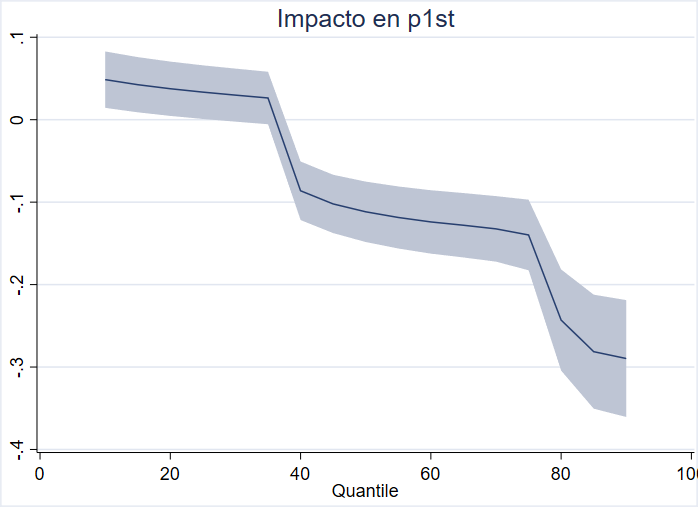
\includegraphics[scale=0.75]{Graph4.png}
\floatfoot{Nota: Se observa el efecto del uso de redes sociales a lo largo de la distribución de la satisfacción con la vida y el intervalo de confianza al 95\%. Para los menos satisfechos con su vida  el impacto del uso de redes sociales es positivo.}
\end{figure}


\subsection{Análisis de sensibilidad}
Como estrategia de sensibilidad se investigó la respuesta del modelo para dos submuestras: los jóvenes de entre 18 y 25 años, y los adultos mayores de 60 años (Cuadro \ref{CyD}). Otros trabajos también realizan ejercicios de sensibilidad con submuestras por edad \cite{Lu2021, Rafnsson2015, Chengbo2014}. 

El primer recorte (jóvenes de entre 18 y 25 años) contabiliza 3.016 observaciones y el segundo (adultos mayores de 60 años) 3.626. Se observa que los jóvenes presentan un mayor nivel de $SWB$ que los adultos (promedio de $sat$ 3.2 contra 2.45. Y promedio de $fel$ 10.31 contra 9.48). 

Para el total muestral se observan en ambos cortes coeficientes negativos, pero mientras que para los adultos mayores de 60 se obtiene un valor de solo -0,591 para los jóvenes alcanza los -6,315. En ambos casos significativo al 1\%. 

En la regresión por cuantiles se mantiene el resultado de un coeficiente positivo para los cuantiles del 25\% y el 50\% y negativo para el cuantil del 75\%. Sin embargo, se pierde la significatividad para los jóvenes. El coeficiente estimado para el cuantil menos felices pasa de 0.15 a 0.35 al restringir la población a solo los adultos mayores de 60 años. Los adultos mayores menos satisfechos con su vida son los que lograron sacar mejor provecho al uso de redes sociales. Probablemente los adultos mayores menos satisfechos con su vida sean de los grupos con menor cantidad de vínculos sociales reales. Especialmente en el contexto de la pandemia donde tuvieron que aislarse para cuidar la salud. Tendría sentido entonces pensar que el uso de redes sociales genere un efecto positivo. Si bien no pueden estar en contacto real con otros, al menos pueden sentirse parte de la comunidad de esta manera. Nuevamente, esto pareciera tener sentido solo porque el vínculo que genera la red social no es en este caso reemplazo de vínculos sociales reales posibles. Estamos haciendo a personas que por aislamiento, por edad y por nivel de $SWB$ muy posiblemente se sientan poco parte de la comunidad.

\begin{table}[htbp]
    \centering
    \caption{Submuestras jóvenes y adultos mayores}
\begin{tabular}{lcccccc} \hline
 & \multicolumn{3}{c}{\makecell{Submuestra\\ jóvenes}} & \multicolumn{3}{c}{\makecell{Submuestra\\ adultos mayores}} \\
 &(1) & (2) & (3) & (4) & (5) & (6) \\
 & ivq25 & ivq50 & ivq75 & ivq25 & ivq50 & ivq75 \\ \hline
 &  &  &  \\
SNU & 0.206 & 0.200 & -0.0184 & 0.350*** & 0.138*** & -0.116** \\
 & (0.127) & (0.124) & (0.0971)  & (0.0688) & (0.0433) & (0.0460) \\
remoto & -0.0199 & -0.0184 & 0.0370 & -0.135** & -0.0912** & -0.0389 \\
 & (0.0427) & (0.0425) & (0.0534) & (0.0640) & (0.0432) & (0.0467)  \\
edad & 0.00259 & 0.00232 & -0.00751 & 0.0110** & 0.00705** & 0.00227\\
 & (0.0120) & (0.0120) & (0.0153) & (0.00498) & (0.00335) & (0.00353)\\
constante & 2.755*** & 2.791*** & 4.110*** & 1.520*** & 2.605*** & 3.910***\\
 & (0.324) & (0.315) & (0.351) & (0.382) & (0.248) & (0.263) \\
 \hline
\end{tabular} 
\label{CyD}
\floatfoot{Nota: Se presenta la salida del modelo de regresiones cuantílicas con variables instrumentales para el caso de los encuestados de entre 18 y 25 años de edad (especificaciones 1 a 3) y para los mayores de 60 años de edad (especificaciones 4 a 6). En la primera fila aparece el estimador del efecto del uso de redes sociales sobre la satisfacción con la vida, correspondiente a la relación causal de interés. Las especificaciones 1 y 4 corresponden a 25\% menos satisfecho con su vida, mientras que las especificaciones 3 y 6 corresponden al 25\% más satisfecho con su vida. Solo los adultos conservan la significatividad del coeficiente en la relación causal de interés. N=3.016 para los jóvenes y N=3.628 para los adultos. Errores estándar robustos entre paréntesis. Kleibergen-Paap = 21.72 (p $<$ 0.01) para los jóvenes y Kleibergen-Paap = 70.08 (p $<$ 0.01) para los adultos. *** p$<$0.01, ** p$<$0.05, * p$<$0.1}
\end{table}

Un análisis por sexo por relega al Anexo. 

\subsection{Chequeo de robustez}
Se propone como chequeo de robustez un cambio sobre la variable objetivo. También se analiza el impacto para cada una de las redes sociales que se incluyen en la variable $SNU$ (Cuadro \ref{por_red}), utilizando la nueva variable objetivo. 

En primer lugar se utiliza como variable objetivo el indicador de felicidad presentado en la sección Datos (\textit{fel}). Toda la investigación realizada para la variable de satisfacción con la vida (\textit{sat}) se repite aquí para la variable felicidad subjetiva (\textit{fel}). El Cuadro \ref{G} equivale al Cuadro \ref{B}, pero para esta nueva variable.

\begin{table}[htbp]
    \centering
    \caption{Felicidad}
\begin{tabular}{lccc} \hline
 & (1) & (2) & (3) \\
VARIABLES & ivq25 & ivq50 & ivq75 \\ \hline
 &  &  &  \\
SNU & 0.247*** & 0.141*** & 0.0264 \\
 & (0.0627) & (0.0535) & (0.0583) \\
p78n & -0.0236 & -0.0877** & -0.158*** \\
 & (0.0474) & (0.0401) & (0.0436) \\
edad & -0.0209*** & -0.0151*** & -0.00879*** \\
 & (0.00154) & (0.00127) & (0.00134) \\
Constant & 8.864*** & 10.58*** & 12.46*** \\
 & (0.134) & (0.110) & (0.122) \\
 &  &  &  \\
 Observations & 19,615 & 19,615 & 19,615 \\ \hline
\multicolumn{4}{c}{ Standard errors in parentheses} \\
\multicolumn{4}{c}{ *** p$<$0.01, ** p$<$0.05, * p$<$0.1} \\
\end{tabular}
 
\label{G}
\floatfoot{Nota: Se presenta la salida del modelo de regresiones cuantílicas con variables instrumentales utilizando como variable objetivo el indicador de felicidad en lugar del de satisfacción con la vida. En la primera fila aparece el estimador del efecto del uso de redes sociales sobre la satisfacción con la vida, correspondiente a la relación causal de interés. La especificación 1 corresponde a 25\% menos feliz, mientras que la especificación 3 al 25\% más feliz. N=11.683 Errores estándar robustos entre paréntesis. Kleibergen-Paap = 348.532 (p $<$ 0.01). *** p$<$0.01, ** p$<$0.05, * p$<$0.1}
\end{table}

El Cuadro \ref{G} presenta la salida de las especificaciones de variables instrumentales cuantílicas para la felicidad (\textit{fel}). Se observa nuevamente un coeficiente para la regresión ordinaria positivo y significativo, que debe considerarse sesgado. Para el total de la muestra también se observa que el coeficiente estimado es negativo y significativo. Y también permanece el efecto positivo y significativo del uso de redes sociales (\textit{SNU}) para el cuantil de los menos felices. La diferencia entonces aparece recién en para los cuantiles del 50\% y del 75\% (especificaciones 2 y 3) que pierden la significatividad. 

Se incluye en la Figura \ref{fig4} la representación del efecto del uso de redes sociales a lo largo de la distribución cuantílica en la felicidad, siguiendo lo ya realizado para la satisfacción con la vida. En la misma se observa que para los más felices el impacto del uso de redes sociales es menor, incluso desaparece. Estos resultados se interpretan como una validación de los resultados principales. El uso de redes sociales muestra un efecto negativo no solo en los niveles de satisfacción con la vida, sino también en otras variables subjetivas de bienestar. Sin embargo, este efecto se revierte entre los menos felices. 

% Figura 4
\begin{figure}[ht]
\centering
\caption{Felicidad}
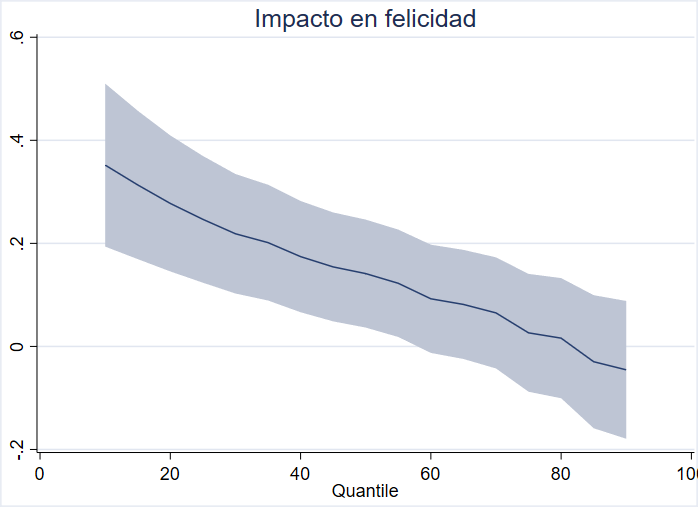
\includegraphics[scale=0.75]{Graph3.png}
\label{fig4}
\floatfoot{Nota: Se observa el efecto del uso de redes sociales a lo largo de la distribución de la felicidad y el intervalo de confianza al 95\%. Para los menos felices el impacto del uso de redes sociales es positivo.}
\end{figure}

El Cuadro \ref{por_red} presenta la estimación del coeficiente para el uso desagregado de cada una de las redes sociales que conforman la variable dummy $SNU$. Las redes más usadas son Whatsapp, Facebook y Youtube. El único caso para el que se pierde la significatividad del efecto positivo del uso de redes sociales en la especificación de los que pertenecen al 25\% menos feliz es Instagram. Esto podría entenderse como una consecuencia del efecto envidia altamente relacionado con esta red social. Incluso, Instagram muestra un efecto negativo y significativo, es decir, caída de la felicidad para el cuantíl de los más felices. La otra red social que genera un efecto negativo significativo es Twitter para el caso de los más felices. Podría pensarse que los más felices que usan Twitter terminan discutiendo con otros, y luego más enojados y menos felices. En cambio, los menos felices lograron simplemente utilizar la red para informarse, dialogar con otros, sentirse parte de la comunidad y lograron así sacarle provecho. Para la mediana, la significatividad se pierde en los casos de Youtube, Twitter y Whatsapp. 

El mayor efecto por uso de red social sobre felicidad se observa en Snapchat y Tiktok. Debe considerarse, sin embargo, que se trata de las dos redes con menor cantidad de usuarios de la encuesta. Podría pensarse también que estas redes tengan un tipo de uso diferente ya que usualmente están dirigidas a un público más joven. 


\begin{table}[htbp]
  \centering
  \caption{Felicidad por Red}
    \begin{tabular}{ccccc}
          & \textbf{ivq25} & \textbf{ivq50} & \textbf{ivq75} & \textbf{Usan red} \\
    \midrule
    \multirow{2}[2]{*}{Total} & 0,198** & 0,100 & -0,00312 & 15573 \\
          & (0,0827) & (0,0709) & (0,0773) &  \\
    \midrule
    \multirow{2}[2]{*}{Facebook} & 0.313*** & 0.206** & 0.0926 & 12842 \\
          & (0.106) & (0.0923) & (0.102) &  \\
    \midrule
    \multirow{2}[2]{*}{Snapchat} & 7.255** & 11.55** & 14.98** & 1710 \\
          & (3.295) & (5.014) & (6.548) &  \\
    \midrule
    \multirow{2}[2]{*}{Youtube} & 0.278* & 0.0506 & -0.189 & 8834 \\
          & (0.158) & (0.144) & (0.162) &  \\
    \midrule
    \multirow{2}[2]{*}{Twitter} & 0.958** & -0.00449 & -0.941** & 2593 \\
          & (0.421) & (0.419) & (0.458) &  \\
    \midrule
    \multirow{2}[2]{*}{Whatsapp} & 0.197** & 0.0838 & -0.0366 & 14394 \\
          & (0.0907) & (0.0781) & (0.0857) &  \\
    \midrule
    \multirow{2}[2]{*}{Instagram} & 0.00665 & -0.490** & -0.950*** & 6155 \\
          & (0.237) & (0.219) & (0.241) &  \\
    \midrule
    \multirow{2}[2]{*}{Tiktok} & 3.130** & 5.585** & 7.572** & 2176 \\
          & (1.361) & (2.510) & (3.524) &  \\
    \midrule
    \multirow{2}[2]{*}{Otro} & 46.60 & 37.82 & 28.82 & 130 \\
          & (167.3) & (137.8) & (107.6) &  \\
    \bottomrule

    \end{tabular}%
  \label{por_red}%
    \floatfoot{Nota: Se presenta la estimación del coeficiente del impacto del uso de redes sociales en la felicidad para los cuantiles seleccionados desagregado por red social. Errores estándar robustos entre paréntesis.  *** p$<$0.01, ** p$<$0.05, * p$<$0.1}
\end{table}%


En el Anexo se incluye un análisis parcial para cada uno de los países incluidos en la encuesta (Cuadro \ref{por_pais}). 

\section{Conclusiones}
El presente trabajo analiza la relación entre el bienestar subjetivo ($SBW$) y el uso de redes sociales ($SNU$) en Latinoamérica en pleno impacto de las consecuencias de la pandemia de COVID-19. Por un lado se investiga el efecto causal, utilizando variables instrumentales, y por otro la variación a lo largo de la distribución de $SBW$ utilizando regresiones cuantílicas. Esto último responde a que se entiende que las personas con mayor bienestar subjetivo hacen un determinado uso de las redes sociales distinto al que hacen las personas con menor bienestar subjetivo, especialmente en un contexto de aislamiento fruto de la pandemia. Si la investigación se basara en los valores promedio, estas diferencias se perderían. Es decir, se hizo uso de un modelo de regresión cuantílica con variables instrumentales (IVQR). 

Los resultados muestran un impacto negativo del uso de redes sociales en el $SWB$ para el total muestral, pero positivo para las personas de menor $SWB$. Esto se interpreta como una predominancia del efecto interacción social por sobre los efectos de envidia social, enviciamiento, pérdida de productividad y otros típicos de la literatura entre los menos felices o satisfechos con su vida. Que las encuestas se hayan realizado durante un período de aislamiento podría dar cuenta de esta predominancia. Es decir, ante la imposibilidad o dificultad de verse presencialmente con familiares y amigos, estas personas sacaron provecho de comunicarse al menos virtualmente con ellos. Esto podría deberse a que los menos felices si no hacen uso de las redes se quedaría sin nada, por su poca interacción social real. 

En el otro extremo de la distribución, puede pensarse que quienes son más felices, tienen mejores vínculos reales, y no necesitan tanto de las redes sociales. El efecto de la interacción social virtual sería así menos importante para los más felices, haciendo que prevalezca el efecto envidia, el distractivo u otros. Los más felices, si no hacen uso de las redes, al menos cuentan todavía con la interacción social real (incluso en el contexto de relativo aislamiento causado por la pandemia), se evitan los efectos negativos y su $SWB$ podría mejorar. 

El trabajo analiza también, como ejercicio de sensibilidad, la respuesta para dos submuestras etarias. Los jóvenes de entre 18 y 25 años, y los adultos mayores de 60 años. En el promedio se observa un efecto negativo para ambos cortes pero mayor para los jóvenes. Esto podría estar vinculado especialmente a efecto envidia. 

En lo que respecta al análisis de cada red social, se observa, en línea con los principales hallazgos del trabajo, que las redes vinculadas al intercambio con personas conocidas y las de uso más común entre jóvenes son las que mayor efecto positivo presentan en $SWB$. Otras, con otros usos típicos, tienen un efecto menor, nulo o negativo. 

Los resultados son robustos a dos especificaciones distintas de $SWB$. Entendiendo este como felicidad subjetiva de acuerdo a la recopilación a distintas respuestas de bienestar personal, económico y social ($fel$) o directamente como la respuesta a la pregunta por satisfacción general con la vida ($sat$). 

Resultaría de interés, para futuras investigaciones, la comparación de estos resultados con otras olas de la encuesta (no vinculadas a los efectos de la pandemia) de manera de especificar el impacto del aislamiento (obligatorio o autoimpuesto) en el vínculo entre el uso de redes sociales y el $SWB$. También restaría identificar las políticas públicas que de mejor manera acerquen el uso de redes sociales a la población de menor $SWB$.

\bibliographystyle{apacite}
\bibliography{biblio}

\newpage
\section{Anexo Metodológico}
Asumiendo integrabilidad, el $\tau$-ésimo cuantíl condicional de $SWB$ dado $X$ resuelve: 

\[Q_{SWB|X} (\tau) \in \argminA_{f \in \mathcal{F}} E[\rho_\tau(SWB-f(X))] \]

Donde $\mathcal{F}$ es la clase de las funciones medibles de $X$.

Por lo tanto, la regresión cuantílica del modelo con variables instrumentales en el $\tau$-ésimo cuantíl de SWB queda identificada por: 

\[ P[SWB_i \leq \alpha_\tau SNU_i + \beta_\tau X_i | X_i Z_i ]= \tau \]

Utilizando la ley de expectativas iteradas (LEI) es posible reemplazar la probabilidad por la esperanza de la función indicadora: 
\[\tau=E[I\{SWB-x' \beta \leq 0 \}|Z]\]

La función objetivo simplificada puede expresarse como: 
\[ arg\,min \sum_{i=1}^{n} \rho_\tau (SWB_i - \alpha_\tau SNU_i - \beta_\tau X_i - \gamma_\tau Z_i) \]

Y la función de perdida cuantílica $\rho_\tau (.)$ queda minimizada por identificación de $\alpha_\tau$.

A diferencia del modelo original, la optimización de la función objetivo de la especificación suavizada (SIVQREG) utiliza estimadores condicionales no paramétricos basados en kernels. El modelo original se resuelve por identificación de $\alpha_\tau$, pero esta identificación no es trivial. Por este motivo \citeA{Kaplan2022} realiza una suavización sobre la función indicadora de manera de convertirla en continua y diferenciable, reemplazando $1\{v\leq 0\}$ por $\Tilde{I} (v)$. De esta manera la función indicadora desciende suavemente de 1 a 0 sobre $-1 \leq v \leq 1$ en vez de en forma discontinua de 1 a 0 cuando $v=0$. También incorpora un ancho de banda $h$ de manera de poder controlar el descenso de $\Tilde{I} (v/h)$ en $-h \leq v \leq h$. El estimador $\hat\beta$ resuelve la condición de momentos suavizada: 

\[ 0=1/n \sum_{i=1}^{n} z_i [\Tilde{I}\{(SWB_i - x_i \hat\beta)/h \}- \tau \]

\newpage
\section{Anexo}
% Figura 1
\begin{figure}[ht]
\centering
\caption{Satisfacción con la vida}

\includegraphics[scale=0.75]{Graph2.png}
\floatfoot{Nota: El gráfico presenta el histograma de la distribución de la satisfacción con la vida superpuesto con la función de densidad de kernel.}
\end{figure}

% Figura 2
\begin{figure}[ht]
\centering
\caption{Felicidad}
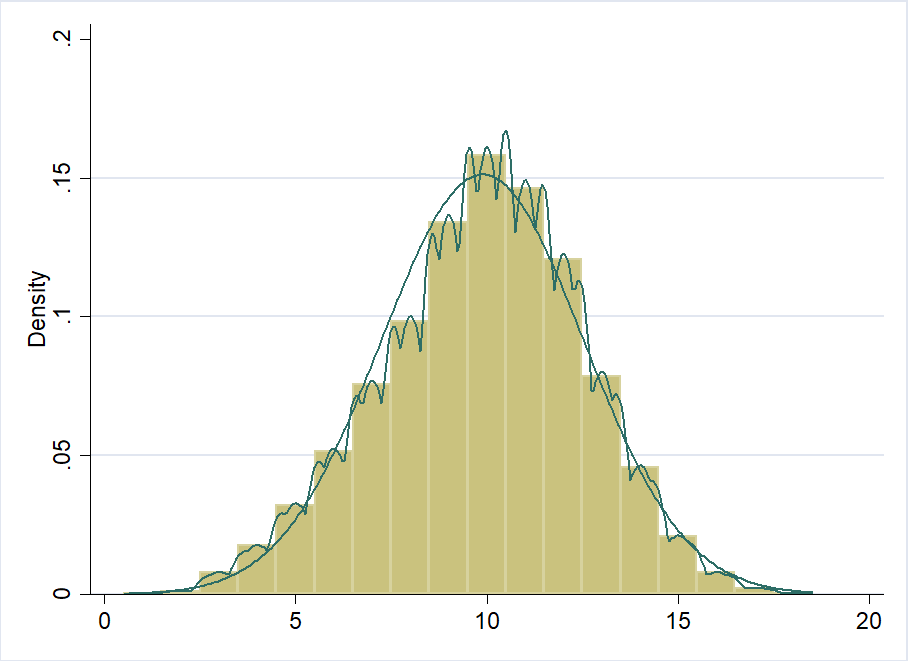
\includegraphics[scale=0.75]{Graph1.png}
\floatfoot{Nota: El gráfico presenta el histograma de la distribución de la felicidad superpuesto con la función de densidad de kernel.}
\end{figure}

Las mujeres representan un 52.43\% de las observaciones, totalizando 6129 entrevistas con datos disponibles. Las mujeres presentan un grado de satisfacción con la vida mayor que los varones. La salida de esta estimación puede observarse en el Cuadro \ref{sexo}. Se mantienen los resultados observados para el total de la población. 

\begin{table}[htbp]
    \centering
    \caption{Submuestra Mujeres}
\begin{tabular}{lccccc} \hline
 &FS & IV & (1) & (2) & (3) \\
 &First-Stage & 2SLS & ivq25 & ivq50 & ivq75 \\ \hline
 & &  &  & & \\
SNU & & -1.1825*** &0.0401 & -0.117*** & -0.156*** \\
 & & (0.2064) &(0.0298) & (0.0341) & (0.0406 \\
remoto & -0.1297*** &  -0.2417*** & 0.0426 & 0.0666*** & 0.0726*** \\
 & (0.0088) & (0.0391) &(0.0265) & (0.0236) & (0.0250) \\
edad & -0.0095*** & -0.0167*** & 0.00602*** & 0.00504*** & 0.00479*** \\
 & (0.0003) & (0.00203) & (0.000700) & (0.000768) & (0.000875) \\
avg\_d\_kbps &  1.78e-06*** & & & & \\
& (1,25e-07) & & & &   \\
constante & 1.3531*** & 5.1107*** & 0.722*** & 1.743*** & 1.997*** \\
 & (0.0183) & (0.2969) & (0.0666) & (0.0669) & (0.0926) \\
  \hline
\end{tabular} 
\label{sexo}
\floatfoot{Nota: Se presenta la salida del modelo de regresiones cuantílicas con variables instrumentales para el caso de las mujeres. En la primera fila aparece el estimador del efecto del uso de redes sociales sobre la satisfacción con la vida, correspondiente a la relación causal de interés. La especificación 1 corresponde a 25\% menos satisfecho con su vida, mientras que la especificación 3 al 25\% más satisfecho con su vida. Se mantienen resultados similares a los obtenidos para el total muestral. n=6.129 Errores estándar robustos entre paréntesis. Kleibergen-Paap = 203.16 (p $<$ 0.01). *** p$<$0.01, ** p$<$0.05, * p$<$0.1}
\end{table}


En el Cuadro \ref{por_pais} se observa el valor del coeficiente de uso de red social (\textit{SNU}) en un análisis individual para cada uno de los países de la encuesta, utilizando \textit{fel} como variable objetivo. Puede observarse así que la mayoría de los países presentan un comportamiento similar al agregado regional. Es decir, un valor del coeficiente estimado para el cuantíl del 25\% menos feliz mayor que los demás. Para varios países, sin embargo, se pierde la significatividad estadística del coeficiente. 


\begin{table}[htbp]
  \centering
  \caption{Felicidad por país}
    \begin{tabular}{cccc}
          & \textbf{ivq25} & \textbf{ivq50} & \textbf{ivq75} \\
    \midrule
    \multicolumn{1}{c}{\multirow{2}[2]{*}{Argentina}} & 0.906 & 0.591 & 0.291 \\
          & (1.003) & (0.965) & (1.153) \\
    \midrule
    \multicolumn{1}{c}{\multirow{2}[2]{*}{Brasil}} & 0.357 & 0.124 & -0.0316 \\
          & (0.352) & (0.293) & (0.306) \\
    \midrule
    \multicolumn{1}{c}{\multirow{2}[2]{*}{Costa Rica}} & 0.130 & 0.489 & 0.769* \\
          & (0.471) & (0.402) & (0.421) \\
    \midrule
    \multicolumn{1}{c}{\multirow{2}[2]{*}{Ecuador}} & 0.429 & 0.393 & 0.361 \\
          & (0.296) & (0.274) & (0.321) \\
    \midrule
    \multicolumn{1}{c}{\multirow{2}[2]{*}{Guatemala}} & 0.195 & -0.189 & -0.492* \\
          & (0.333) & (0.279) & (0.296) \\
    \midrule
    \multicolumn{1}{c}{\multirow{2}[2]{*}{México}} & 0.396 & 0.608** & 0.857*** \\
          & (0.305) & (0.271) & (0.311) \\
    \midrule
    \multicolumn{1}{c}{\multirow{2}[2]{*}{Panamá}} & -0.876 & -0.822 & -0.792 \\
          & (0.870) & (0.619) & (0.574) \\
    \midrule
    \multicolumn{1}{c}{\multirow{2}[2]{*}{Perú}} & 0.415* & 0.478** & 0.538** \\
          & (0.229) & (0.199) & (0.218) \\
    \midrule
    \multicolumn{1}{c}{\multirow{2}[2]{*}{Uruguay}} & 0.619* & 0.367 & 0.157 \\
          & (0.345) & (0.288) & (0.302) \\
    \midrule
    \multicolumn{1}{c}{\multirow{2}[2]{*}{Bolivia}} & 0.204 & 0.178 & 0.151 \\
          & (0.247) & (0.215) & (0.235) \\
    \midrule
    \multicolumn{1}{c}{\multirow{2}[2]{*}{Colombia}} & -0.310 & -0.240 & -0.188 \\
          & (0.316) & (0.253) & (0.249) \\
    \midrule
    \multicolumn{1}{c}{\multirow{2}[2]{*}{Chile}} & 0.987** & 1.044*** & 1.105*** \\
          & (0.420) & (0.352) & (0.348) \\
    \midrule
    \multicolumn{1}{c}{\multirow{2}[2]{*}{El Salvador}} & 1.228*** & 1.024*** & 0.812*** \\
          & (0.364) & (0.285) & (0.287) \\
    \midrule
    \multicolumn{1}{c}{\multirow{2}[2]{*}{Honduras}} & -0.0310 & -0.224 & -0.385 \\
          & (0.577) & (0.420) & (0.384) \\
    \midrule
    \multicolumn{1}{c}{\multirow{2}[2]{*}{Nicaragua}} & 1.323*** & 0.881*** & 0.551** \\
          & (0.312) & (0.257) & (0.270) \\
    \midrule
    \multicolumn{1}{c}{\multirow{2}[2]{*}{Paraguay}} & 0.311 & 0.277 & 0.251 \\
          & (0.381) & (0.333) & (0.353) \\
    \midrule
    \multicolumn{1}{c}{\multirow{2}[2]{*}{República  Dominicana}} & -0.000166 & -0.136 & -0.292 \\
          & (0.376) & (0.321) & (0.346) \\
    \midrule
    \multicolumn{1}{c}{\multirow{2}[2]{*}{Venezuela}} & -0.276 & -0.680** & -1.103*** \\
          & (0.258) & (0.271) & (0.347) \\
    \bottomrule

    \end{tabular}%
  \label{por_pais}%
  \floatfoot{Nota: Se presenta la estimación del coeficiente del impacto del uso de redes sociales en la felicdad para los cuantiles seleccionados desagregado por país. Errores estándar robustos entre paréntesis.  *** p$<$0.01, ** p$<$0.05, * p$<$0.1}
\end{table}%



\end{document}